\begin{problem}{Сопротивление бесполезно!}{input.txt}{output.txt}{2 секунды}{256 мегабайт}

Мальчик Антоша учится в 8 классе гимназии №42 города Гепардовска. Он недавно проходил по физике электрические цепи и резисторы. Антоша собрал схему, состоящую из $n$ резисторов. Пронумеруем их целыми числами от $1$ до $n$ слева направо. $i$-й резистор имеет сопротивление $a_i$ Ом.

Известно, что если в схеме рядом стоят два резистора, имеющие одинаковое сопротивление, то схема взрывается. Такого нельзя допускать. Изначально никакие два резистора с одинаковым сопротивлением в схеме не стояли рядом.

Клон Антоши, мальчик Антоша++, тоже хочет собрать свою схему из резисторов. Но для начала ему надо разобрать схему Антоши. Антоша++ может извлекать резисторы из схемы по одному. При этом важно, чтобы после удаления очередного резистора схема не взорвалась, то есть никакие два резистора с одинаковым сопротивлением не должны стоять рядом после каждого такого удаления. Например, после удаления из схемы с резисторами $[2, 1, 2]$ второго резистора образуется взрывоопасная схема $[2, 2]$, поэтому такое удаление запрещено. В то же время, из схемы $[1, 2, 3, 4, 5, 6]$ можно удалить резистор $5$ и получить безопасную схему $[1, 2, 3, 4, 6]$.

Антоша++ силен в комбинаторике, поэтому решил узнать: а сколько существует способов удалить все резисторы согласно описанным выше правилам? Два способа считаются различными, если на каком-либо шаге позиции удаляемых резисторов различаются.

Он уже пять часов не может решить эту задачу, поэтому Вам необходимо помочь Антоше++ и решить ее. Поскольку ответ может быть огромным, необходимо вывести его по модулю $998244353$, то есть найти остаток от деления ответа на магическое число $998244353$.

\begin{center}
	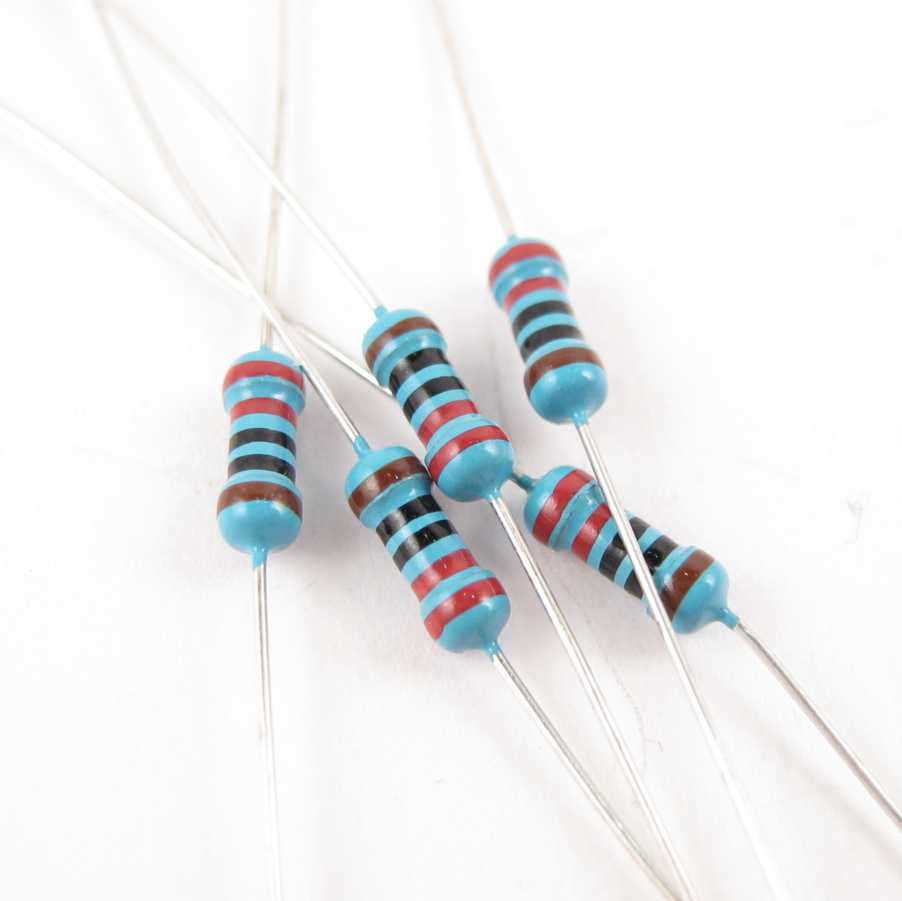
\includegraphics[width=0.4\textwidth]{task3.png}
	
	\scriptsize \textit{Источник:} \t{https://uscr.ru/rezistor/}
\end{center}

\InputFile

В первой строке входных данных находится целое число $n$ ($1 \le n \le 500$)~--- количество резисторов в схеме Антоши.

Во второй строке входных данных находится $n$ целых чисел $a_i$ ($1 \le a_i \le n$)~--- сопротивление $i$-го резистора.

Гарантируется, что никакие два резистора с одинаковым сопротивлением не стоят рядом.

\OutputFile

Выведите одно целое число~--- ответ на задачу по модулю $998244353$. Если Вы выведете число, не являющееся ответом на задачу, то Вы получите вердикт <<Неправильный ответ>>, а Антоша++ обидится на Вас.

\Examples

\begin{example}
\exmp{
3
1 2 3
}{
6
}%
\exmp{
4
1 2 1 2
}{
8
}%
\exmp{
12
1 2 3 1 2 3 1 2 3 1 2 3
}{
25660800
}%
\exmp{
1
1
}{
1
}%
\end{example}

\Scoring

В этой задаче \textbf{потестовая оценка}. Тесты условно разбиты на подзадачи, за полное прохождение всех тестов подзадачи начисляются соответствующие ей баллы. Подзадачи приведены в следующей таблице:

\medskip

\begin{tabular}{| c | c | c |} \hline
	№ & Ограничения & Баллы за подзадачу \\ \hline
	1 & $n \le 9$ & 10 \\ \hline
	2 & $a_i \le 2$ & 10 \\ \hline
	3 & $n \le 20$ & 20 \\ \hline
	4 & $n \le 100$ & 30 \\ \hline
	5 & Нет дополнительных ограничений & 30 \\ \hline
\end{tabular}

\end{problem}

